\chapter{実験}
\label{chap:result}
\fancyhf{}
\rhead{\thepage}
\lhead{第\ref{chap:result}章 実験}
\cfoot{\thepage}


本章では,実験について述べる.
まず,データセットへの適合のためのDeep Knowledge Tracingの拡張法を述べたのち,
次に,実験設定について述べ,
その後,実験結果について述べる.
実験結果においては,
まず,11データセットのいずれのデータセットにおいても,
Deep Knowledge Tracingの予測性能が知識間関係を考慮しないBayesian Knowledge Tracingよりも高いことを示し,
Deep Knowledge Tracingにより知識獲得における知識間関係を抽出できていることを定量的に確認する.
さらに,
11の知識間関係ネットワークを可視化し,
ネットワーク全体におけるノード集合の配置やその関係を内容の側面から分析し,
知識獲得における知識間関係を抽出できていることを定性的に確認する.
そして,
宣言的知識の知識構造を表現する5つのネットワークと
手続き的知識の知識構造を表現する6つのネットワーク
のモジュラリティとフロー階層,GRCを算出し,
知識獲得における知識構造について,
宣言的知識のモジュール性が手続き的知識のモジュール性より統計的に有意に高く,
逆に,
手続き的知識の階層性が宣言的知識の階層性より統計的に有意に高いことを示す.


\section{Deep Knowledge Tracingの拡張および最適化}
データセットへの適合のためのDeep Knowledge Tracingの拡張法を述べ,その後その最適化について述べる.
勉強サプリの問題演習は
テスト形式で提供されており,一度に1つ以上の問題が提供され,また,それらの採点も同時に行われるため,
同時に複数の問題の回答ログデータが発生する可能性があり,
同時に1つの問題しか回答ログデータが発生しないというDeep Knowledge Tracingで想定されている設定と異なる.
そのため,
Deep Knowledge Tracingをデータセットに適合するように拡張する.


Knowledge Tracingは
学習者の時刻$t$において観測された問題回答結果を$q_{t}$とすれば,
$q_1, q_2, \dots, q_t$から時刻$t+1$において観測される問題回答結果$q_{t+1}$を予測するタスクであった.

同時に複数の問題について回答ログが生じることを許容する場合, 
Knowledge Tracingのタスクは
学習者の時刻$t$において観測された問題回答結果ベクトルを${\bf q}_{t}$とすれば,
${\bf q}_1, {\bf q}_2, \dots, {\bf q}_t$から時刻$t+1$において観測される問題回答結果ベクトル${\bf q}_{t+1}$を予測するというものである.

Deep Knowledge TracingではRNNへの入力はone-hotベクトルに符号化され,入力ベクトルを${\bf x}_t$,
演習問題の数を$M$とすれば,${\bf x}_t$の長さは$2M$であった.
同時に複数の問題が回答されるという設定では,
その同時に回答された問題数を$m_t$とすれば$m_t$-hotベクトルに符号化することで,
\cite{piech2015deep}に近い形でRNNに情報を入力できる.

\begin{table}[ht]
\caption{拡張したDeep Knowledge Tracingにおける回答ログデータと対応する入力ベクトルの例}
\label{tab:samplelog_mod}
\begin{center}
\centerline{
{
\begin{tabular}{crrr|cc}\hline\hline
	\multicolumn{4}{c|}{回答ログ}	&	\multicolumn{2}{c}{入力ベクトル}	\\
	ユーザID	&	ログの順番	&	問題番号	&	正誤	&	変数名			&	値											\\\hline
	A			&	1			&	1			&	1		&	\multirow{2}{*}{${\bf x}_1$}		&	\multirow{2}{*}{$[1 0 0 0 \vdots 0 1 0 0 ]$}	\\
	A			&	1			&	2			&	0		&					   	 	&												\\\hdashline
	A			&	2			&	1			&	1		&	\multirow{2}{*}{${\bf x}_2$}		&	\multirow{2}{*}{$[1 1 0 0 \vdots 0 0 0 0 ]$}	\\
	A			&	2			&	2			&	1		&					   	 	&												\\\hdashline
	A			&	3			&	3			&	0		&	${\bf x}_3$					&	$[0 0 0 0 \vdots 0 0 1 0 ]$			\\\hdashline
	A			&	4			&	3			&	0		&	\multirow{2}{*}{${\bf x}_4$}	&	\multirow{2}{*}{$[0 0 0 1 \vdots 0 0 1 0 ]$}											\\
	A			&	4			&	4			&	1		&							&												\\
\hline\hline
\end{tabular}
}
}
\end{center}
\end{table}

具体例を交えて説明する.
例えば,演習問題の数が4つと仮定する .$M=4$であり,${\bf x}_t$の長さは$8$である.
ある学習者が,表\ref{tab:samplelog_mod}の回答ログのように問題を回答し正誤が観測されたとすれば,
入力ベクトル${\bf x}_t$は表\ref{tab:samplelog_mod}の入力ベクトルのように符号化される.

出力${\bf y}_t$はDeep Knowledge Tracingと全く同じであり,
問題と同じ長さのベクトルで,
それぞれの要素が当該学習者がそれぞれの問題に正しく回答する確率の予測値となっている.
したがって,$t+1$の回答${\bf q}_{t+1}$の正誤予測は$t+1$に回答される問題${\bf q}_{t+1}$に対応する${\bf y}_t$の要素から読み取れる.

最適化手法は\cite{piech2015deep}のものとほとんど同じである.
\begin{eqnarray}
	\log(p_1 \times p_2 \times \dots \times p_{m_t}) = \sum_{k}^{m_t} \log(p_k)
\end{eqnarray}
であるため,
${\bf\tilde{ \delta}}({\bf q}_{t+1})$を時刻$t+1$にどの問題が回答されたかの$m_t$-hotベクトルとし,
${\bf a}_{t+1}$を時刻$t+1$に対応する問題で正答したか否か($1$か$0$)のベクトルとすれば,
ロス関数は
\begin{eqnarray}
L &=& \sum_t l({\bf y}_t^T {\bf \tilde{\delta}}({\bf q}_{t+1}), {\bf a}_{t+1})
\end{eqnarray}
である.
学習時は\cite{piech2015deep}と同様にミニバッチごとに確率的勾配降下法で目的関数を最小化する.

ハイパーパラメタについては,
対象データが多いため学習コストの削減を狙いRNNの部分にはGRNNを用いる.
学習率の初期値を$200$,
モーメントを$0.98$,
1エポックごとに,
減衰率$0.8$として学習率を最小学習率$10$まで減衰させる.
また,勾配のノルムの最大値を$0.00001$として\cite{pascanu2013difficulty}に従い勾配に制約を設けた.
dropoutは\cite{piech2015deep}と同様に${\bf y}_t$の方向にのみかけ,
dropout率は$0.5$とした.
隠れ層のユニット数は$200$として,
各重み行列の初期化は\cite{glorot2010understanding}にしたがった.
時系列方向の誤差逆伝搬は最長で$200$まで伝搬するように制約を設けた.

これらのハイパーパラメタは実験的に高い予測性能を発揮したため設定しており,
網羅的に探索したわけではない.
通常,深層学習の手法はハイパーパラメタの数が非常に大きく,また,
計算コストが大きいため大規模な探索は行えない.
Grid SearchやRandom Search\cite{bergstra2012random}といった探索手法が提案されているが,
専門家が手で調整した方が優れていることが報告されている\cite{larochelle2007empirical, bergstra2012random}
.

実装には
Theanoを用いた\cite{bergstra+al:2010-scipy,Bastien-Theano-2012}.
Theanoは多次元行列を含む数学的表現の定義や計算,最適化を効率的に行えるPythonのライブラリで,
深層学習の研究ではよく利用される.


以上,Deep Knowledge Tracingの拡張およびその最適化について述べた.
次に,実験設定について述べる.

\section{設定}
ここでは,
特にDeep Knowledge Tracingによる知識獲得の予測の実験設定,
および,
構築したネットワークの可視化の設定,ネットワーク構造指標の計算について述べる.


まず,Deep Knowledge Tracingによる知識獲得の予測の実験設定について,
11のデータセットそれぞれについて,
訓練:検証:テスト = 8:1:1となるようにユーザを分け,
訓練ユーザのデータでモデルを構築し,
検証ユーザのデータでハイパーパラメタを調整し, 
検証ユーザのデータで精度が最も高かったモデルを
テストユーザのデータに適用し当該モデルの最終的な精度とする.
小学生や中学生が学習する内容は国が定める学習指導要領\cite{gakushushidouyouryou}に従っており,
学習内容が高い頻度で入れ替わっていくというわけではないため,
勉強サプリの学習教材もまた,更新頻度は高くない.
したがって,
Knowledge Tracingのモデルは
商品推薦や広告推薦の領域でしばしば問題となるアイテムに関するコールドスタート問題\cite{schein2002methods}の影響を受けにくく,
こうして同じ時期のユーザを分割する評価方法でもモデルの性能を十分評価できると考えられる.


次に,
構築したネットワークの可視化の設定およびネットワーク構造指標の計算について述べる.
ネットワークの可視化にはGephi\cite{bastian2009gephi}を用いた.
Gephiはネットワーク可視化用のソフトウェアであり,
豊富なレイアウト手法やネットワークの統計量計算ツールが提供されている.
ノードは問題を,エッジは影響関係を示すように可視化する.
ノードの色はデータセットの説明の際に用いた平均問題着手番号について,番号が小さいものから大きいものにかけて青色から赤色になるようにする.
ノードの大きさはノードの出力次数に比例するように可視化する.
ノードのラベルはそのノードが指す問題が提供される授業名とその問題に割り振った適当な数字を結合した文字列を利用する.
また,一見してクラスタだと判断できそうなノード集合には,ノードやその結合が分かりにくくならない範囲で扱われている内容の説明を近くに記載する.
ネットワークのレイアウト手法には,ForceAtlas\cite{jacomy2009force}を用いる.
また,モジュラリティの計算はGephiで行い,
フロー階層とGRCの計算はNetworkX\cite{hagberg-2008-exploring}というネットワーク解析や探索及びネットワークアルゴリズムを提供するPythonのライブラリを用いた.



以上,実験設定について述べた.
次に,実験結果について述べる.


\section{結果}
実験結果について述べる.
まず,11データセットのいずれのデータセットにおいても,
Deep Knowledge Tracingの予測性能が知識間関係を考慮しないBayesian Knowledge Tracingよりも大きく高いことを示し,
Deep Knowledge Tracingにより知識獲得における知識間関係を抽出できていることを定量的に確認する.
さらに,
11の知識間関係ネットワークを可視化し,
ネットワーク全体におけるノード集合の配置やその関係を内容の側面から分析し,
知識獲得における知識間関係を抽出できていることを定性的に確認する.
そして,
宣言的知識の知識構造を表現する5つのネットワークと
手続き的知識の知識構造を表現する6つのネットワーク
のモジュラリティとフロー階層,GRCを算出し,
知識獲得における知識構造について,
宣言的知識のモジュール性が手続き的知識のモジュール性より統計的に有意に高く,
逆に,
手続き的知識の階層性が宣言的知識の階層性より統計的に有意に高いことを示す.


\subsection{各データセットにおける予測性能}
\begin{table}[!htb]
\caption{各データセットに対する各手法の予測性能とそれらの関係性}
\label{tab:result1}
\begin{center}
\centerline{
{
\begin{tabular}{ccc|rrr|cc}\hline\hline
\multicolumn{3}{c|}{データセット}	&	\multicolumn{3}{c|}{AUC}	& \multicolumn{2}{c}{DKT $-$ BKT}\\
分類	& 科目			&				学年			&	Marginal&	BKT		&	DKT			&	値		&	平均\\\hline
\multirow{5}{*}{\shortstack{宣言的知識\\の獲得を\\主目的とする\\データセット}}&	\multirow{3}{*}{地理・社会}		&				小学4年			&	0.701	&	0.739	&	0.791		&	0.052	&	\multirow{5}{*}{\bf 0.086}	\\
	&			&	小学5年			&	0.647	&	0.680	&	0.765		&	0.085	&		\\	
		&				&				中学			&	0.655	&	0.681	&	0.764		&	0.083	&		\\\cdashline{2-7}
		&\multirow{2}{*}{歴史・社会}	&	小学6年			&	0.642	&	0.657	&	0.773		&	{\bf 0.116}	&		\\	
		&				&				歴史			&	0.635	&	0.670	&	0.766		&	0.096	&		\\\hdashline
%
\multirow{6}{*}{\shortstack{手続き的知識\\の獲得を\\主目的とする\\データセット}}&		\multirow{6}{*}{算数・数学}&	小学4年			&	0.696	&	0.707	&	{\bf 0.828}	&	{\bf 0.121}	&	\multirow{6}{*}{\bf 0.082}	\\	
		&				&				小学5年			&	0.714	&	0.724	&	{\bf 0.804}	&	0.081	&		\\	
		&				&				小学6年			&	0.734	&	0.749	&	{\bf 0.836}	&	0.087	&		\\	
		&				&				中学1年			&	0.738	&	0.750	&	{\bf 0.807}	&	0.057	&		\\	
		&				&				中学2年			&	0.675	&	0.696	&	0.773		&	0.077	&		\\   
		&				&				中学3年			&	0.729	&	0.735	&	{\bf 0.804}	&	0.069	&		\\
%	
\hline\hline
\end{tabular}
}
}
\end{center}
\end{table}

Deep Knowledge Tracing(以下,DKT)とBayesian Knowledge Tracing(以下,BKT)を11データセットに適用した結果を表\ref{tab:result1}に示す.
Marginalは各問題についてそれぞれ正解の周辺確率を予測結果とするものである.
\cite{piech2015deep}にも記載されていたため,本稿でも同様にベースラインとして記載した.
また,
値が大きい箇所は太字で記載した.

まず,すべてのデータセットにおいてDKTのAUCはBKTのAUCよりも大きく高かった.
また,DKT$-$BKTの値の平均も 
宣言的知識の獲得を主目的とするデータセットと
手続き的知識の獲得を主目的とするデータセットで
ほとんど差はなかった.
つまり,
宣言的知識の獲得を主目的とするデータセットと
手続き的知識の獲得を主目的とするデータセットともに,
DKTにより知識獲得における知識間関係を抽出できていると考えられる.

次に,特に,算数や数学の6つのデータセットにおいて,
中学2年のデータセットを除く5つのデータセットにおいてDKTのAUCは0.8を超えており,
\cite{piech2015deep}で示されたように,確かに,DKTが数学のデータセットに対して有効であった.
地理や歴史の社会関係のデータセットにおいてもDKTのAUCは0.76を超えており,
DKTが地理や歴史の社会関係のデータセットに対して有効であり,
宣言的知識の獲得を主目的とするデータセットに対しても有効であることが示された.


以上,
11データセットのいずれのデータセットにおいても,
Deep Knowledge Tracingにより知識獲得における知識間関係を抽出できていることを確認した.




\subsection{抽出した知識間関係ネットワークの可視化}
11の知識間関係をネットワークとして可視化し,
ネットワーク全体におけるノード集合の配置やその関係を内容の側面から分析し,
これらのネットワークが,
知識獲得における知識構造を表現しているものであることを定性的に確認する.




まず,
宣言的知識について知識間関係ネットワークを順に可視化していく.

\subsubsection{小学4年社会}
\begin{figure}[!htb]
\begin{center}
	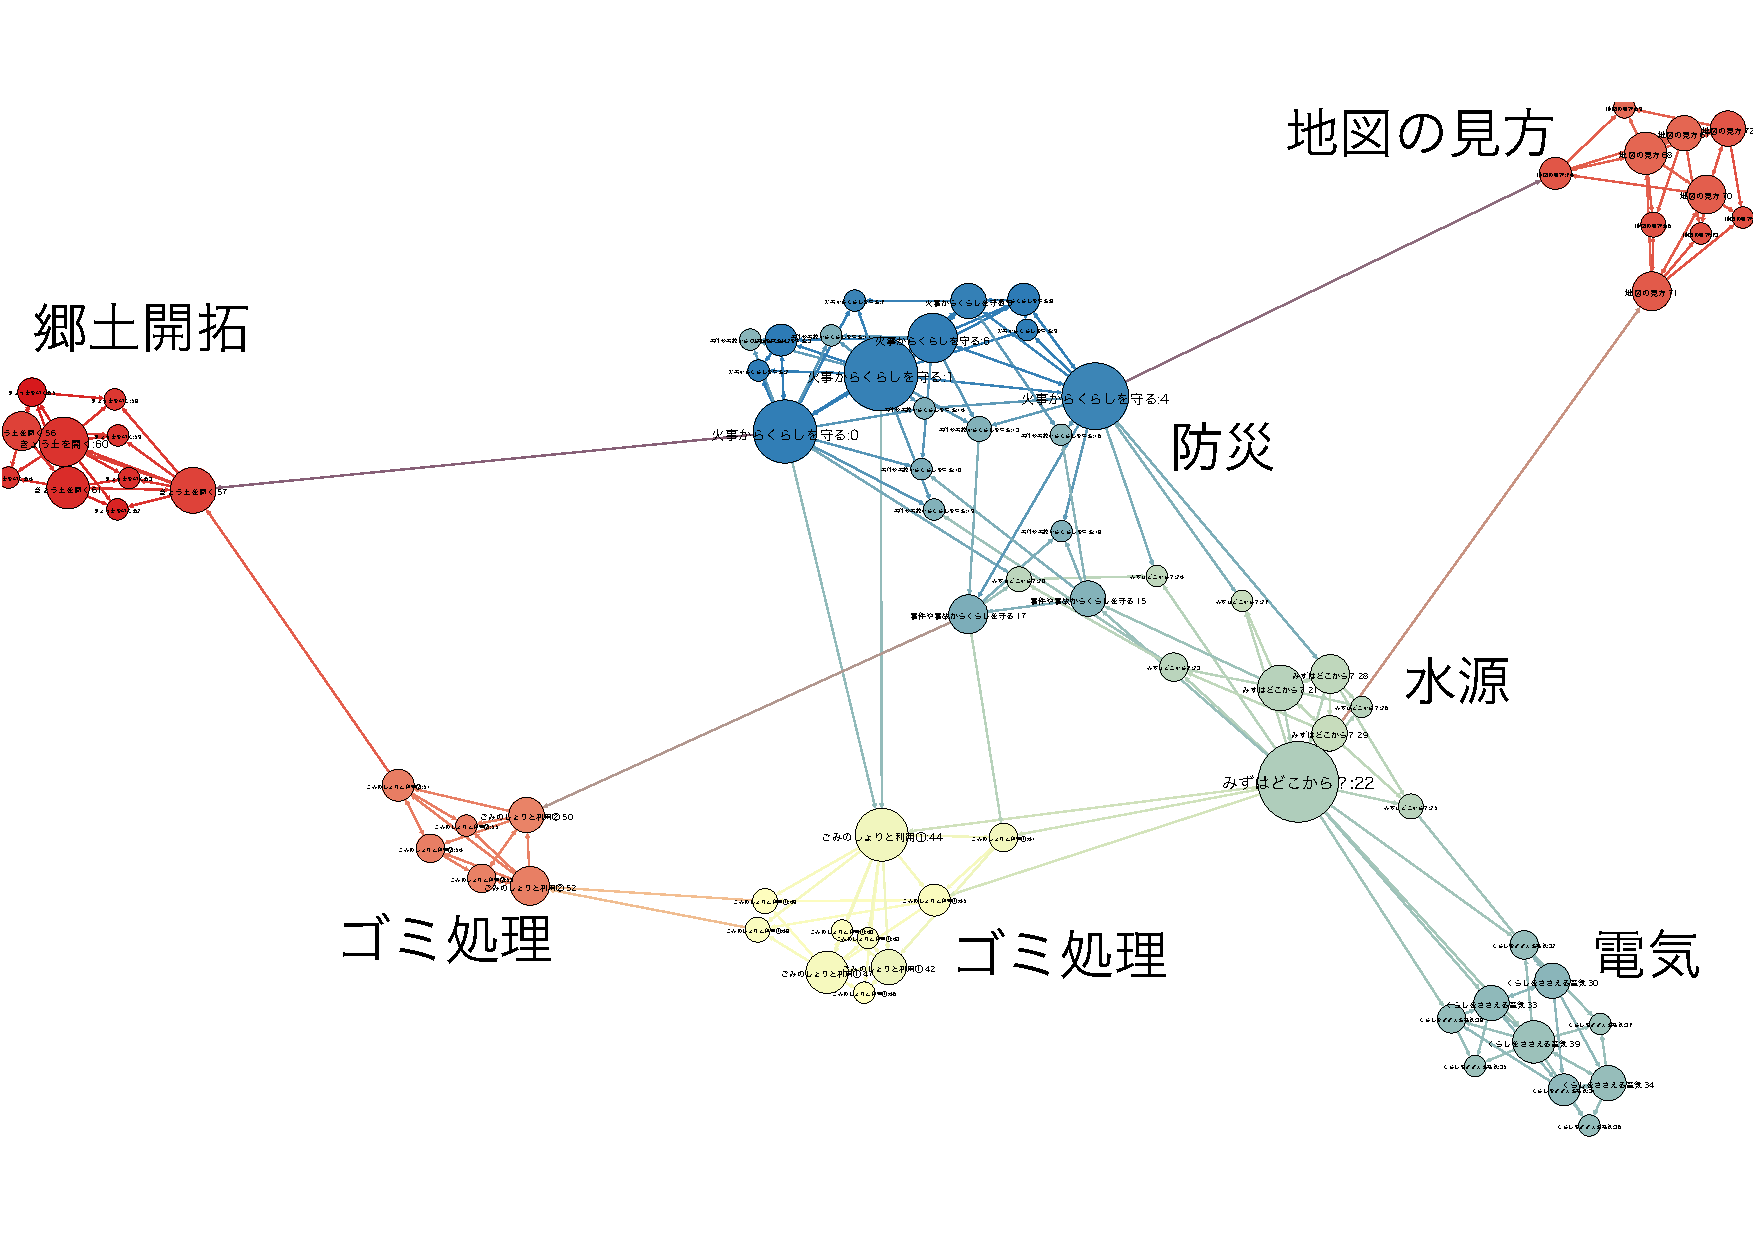
\includegraphics[width=330pt]{./img/s4_soc_label2.pdf}
	\caption{小学4年社会の知識間関係ネットワーク}
	\label{fig:net_s4soc}
\end{center}
\end{figure}
小学4年社会のネットワークを図\ref{fig:net_s4soc}に示す.
ノードは内容ごとでクラスタを形成していることが分かる.
クラスタ間の関係は弱い関係となっていそうである.
特筆すべき点は,防災とラベル付けしたクラスタは火事に関するものと事故や事件に関するものが1つとなってできているということである.






\subsubsection{小学5年社会}
\begin{figure}[!htb]
\begin{center}
	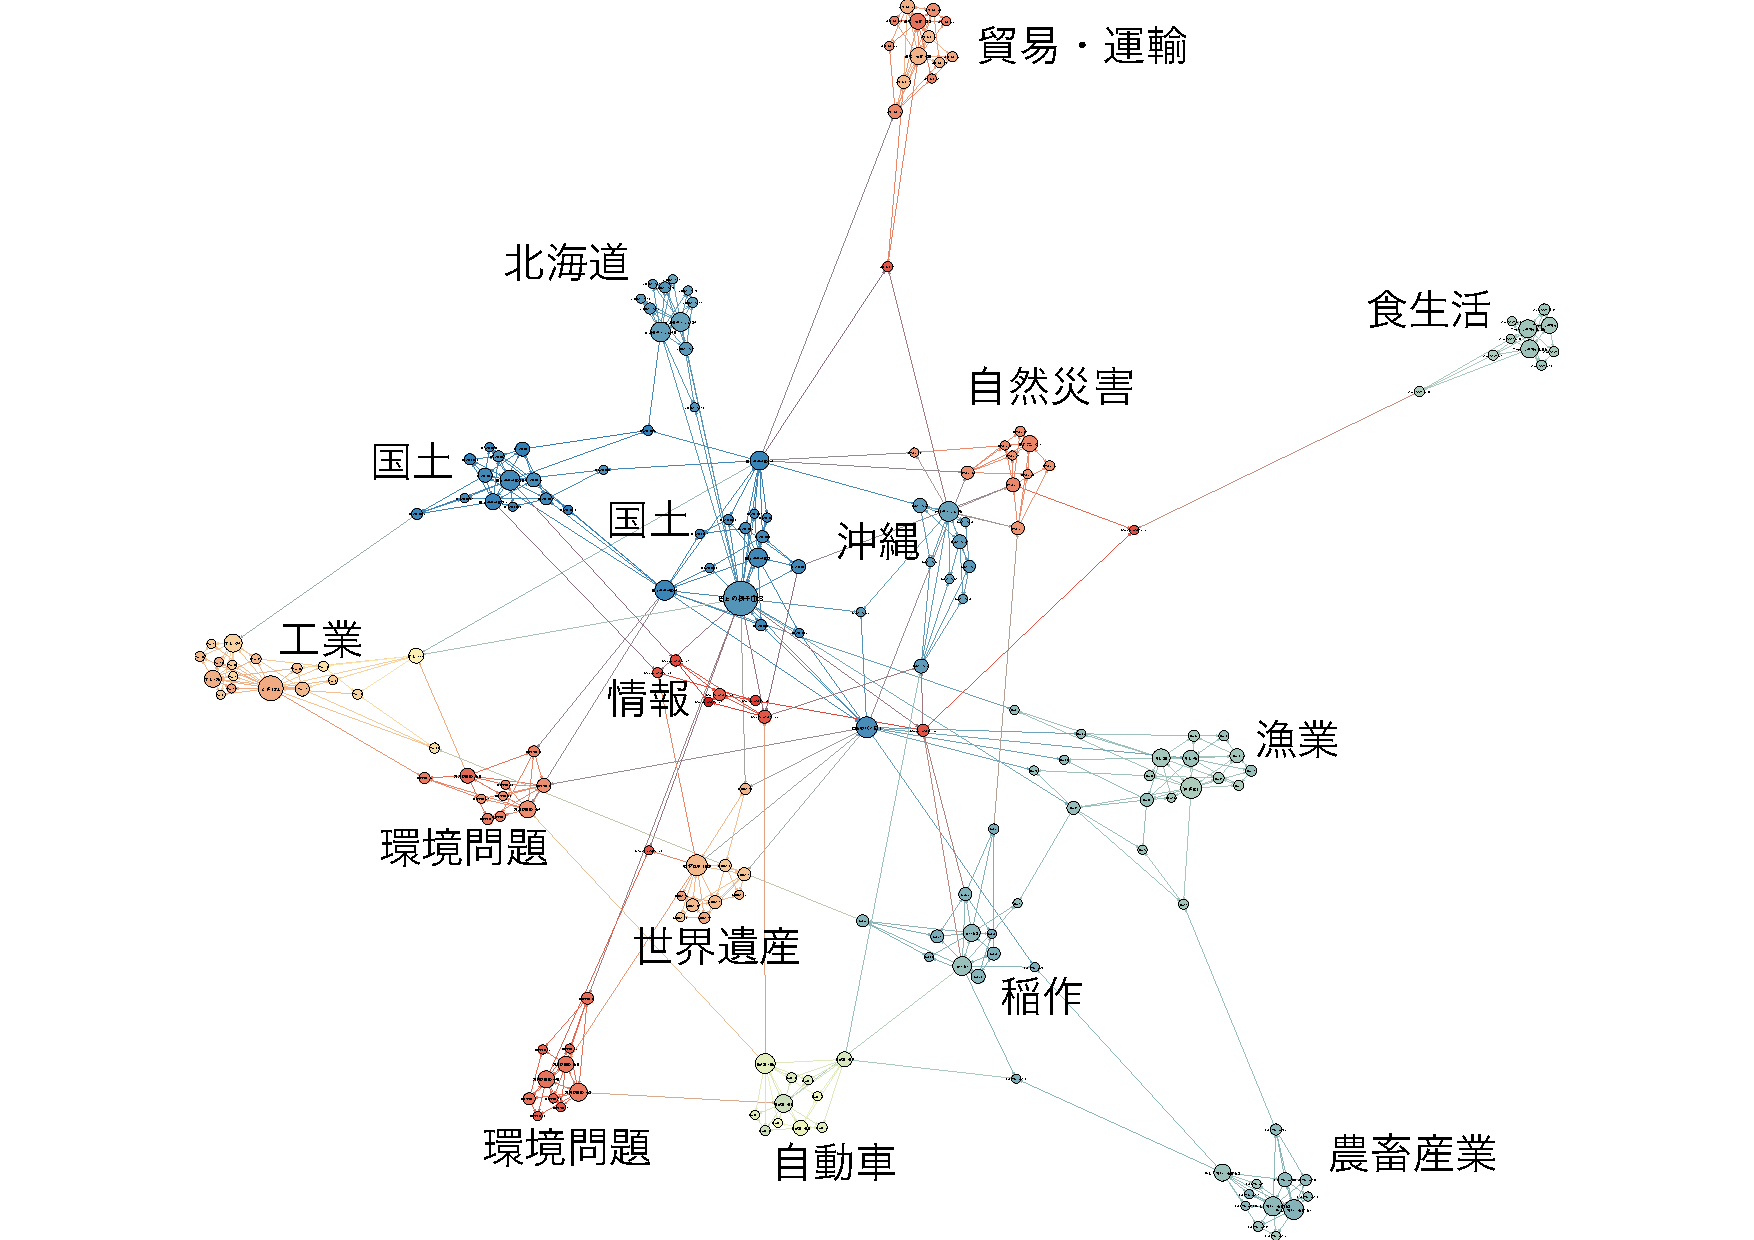
\includegraphics[width=330pt]{./img/s5_soc_label2.pdf}
	\caption{小学5年社会の知識間関係ネットワーク}
	\label{fig:net_s5soc}
\end{center}
\end{figure}
小学5年社会のネットワークを図\ref{fig:net_s5soc}に示す.
ノードは内容ごとでクラスタを形成している.
特に,国土,北海道,沖縄のクラスタが近くにあることは,国土における地理関係において北海道と沖縄の関連が強いからだと考えられる.
また,工業と近い環境問題と自動車と近い環境問題があることも,それぞれの文脈において環境問題があることと関連がある可能性がある.

\subsubsection{小学6年社会}
\begin{figure}[!htb]
\begin{center}
	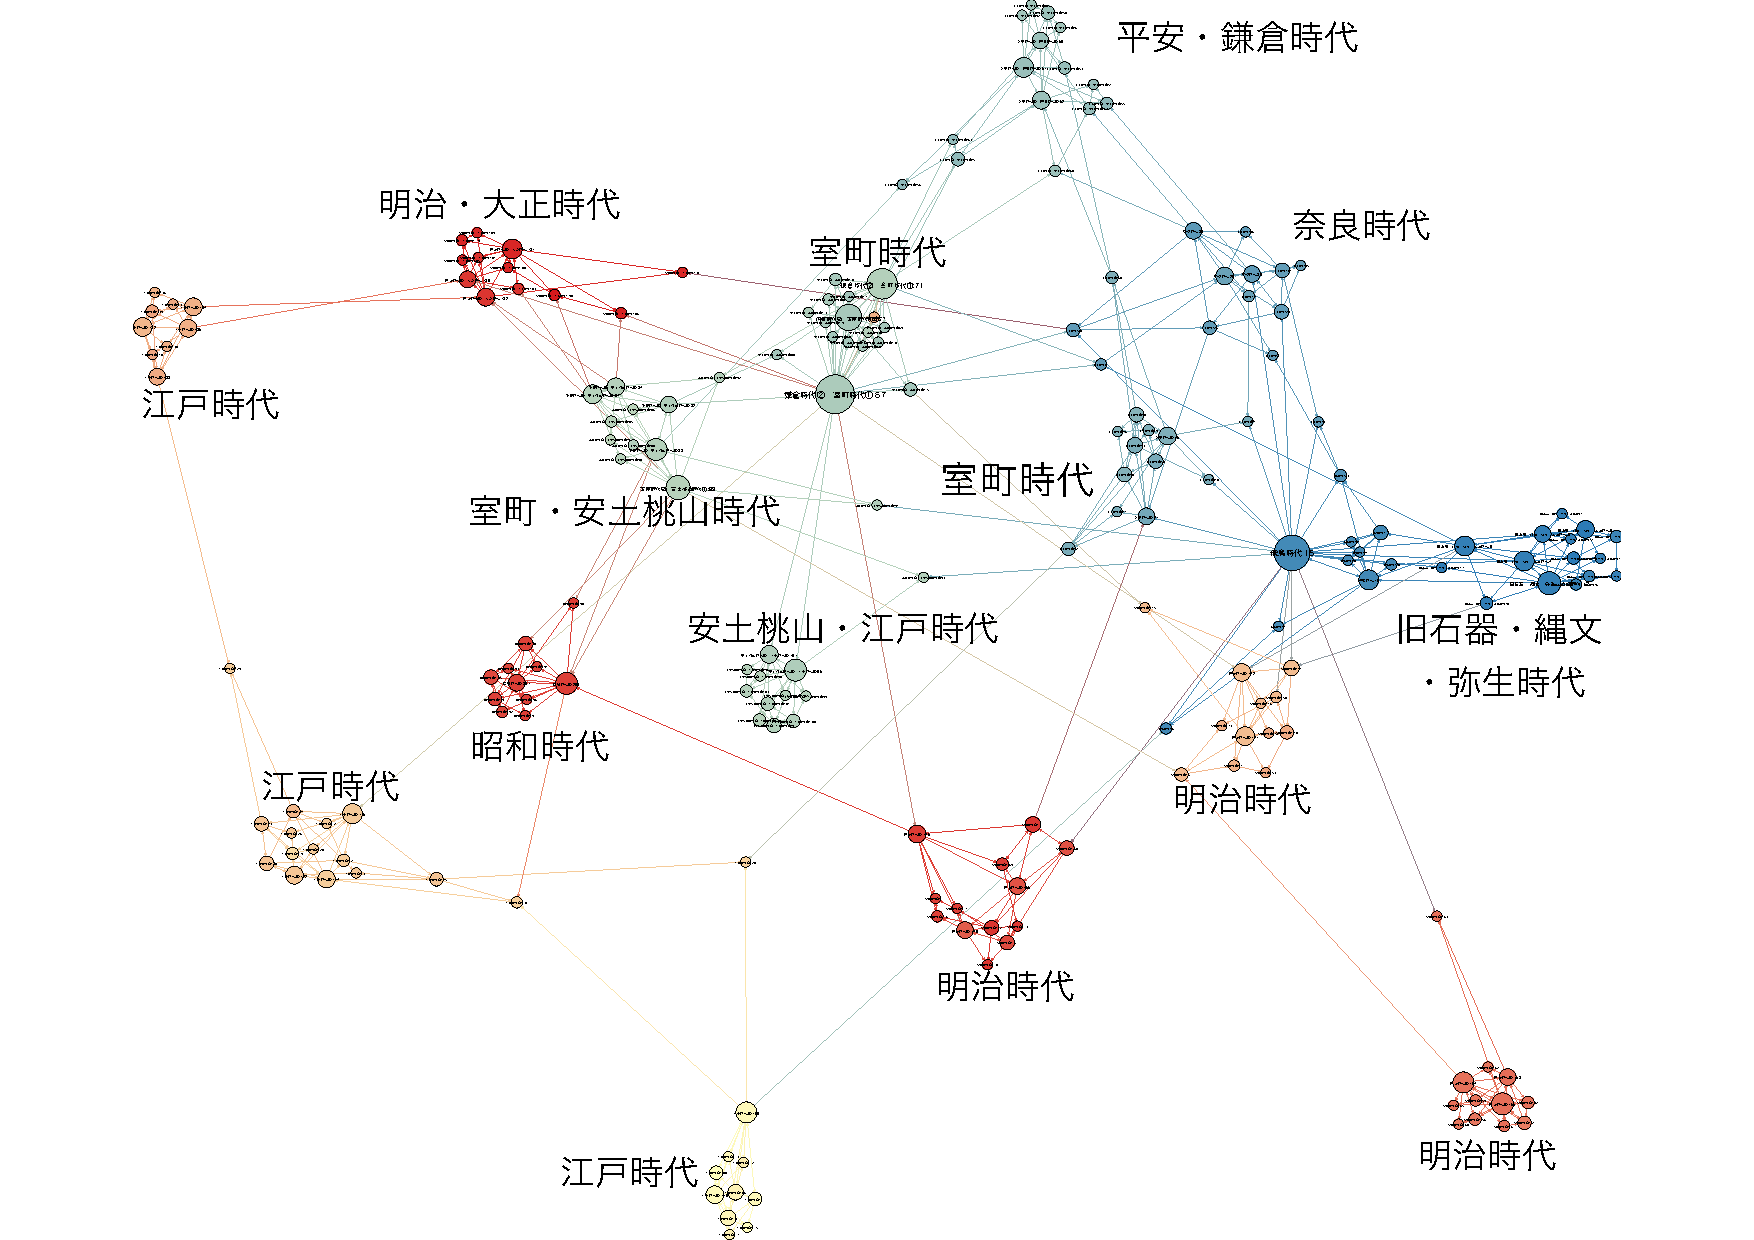
\includegraphics[width=330pt]{./img/s6_soc_label2.pdf}
	\caption{小学6年社会の知識間関係ネットワーク}
	\label{fig:net_s6soc}
\end{center}
\end{figure}
小学6年社会のネットワークを図\ref{fig:net_s6soc}に示す.
ノードは内容ごとでクラスタを形成している.
特に,
クラスタは各時代を表現しているが,逆に,江戸時代や明治時代等の一部の時代は1つのクラスタを形成しているというわけではない.


\subsubsection{中学地理}
\begin{figure}[!htb]
\begin{center}
	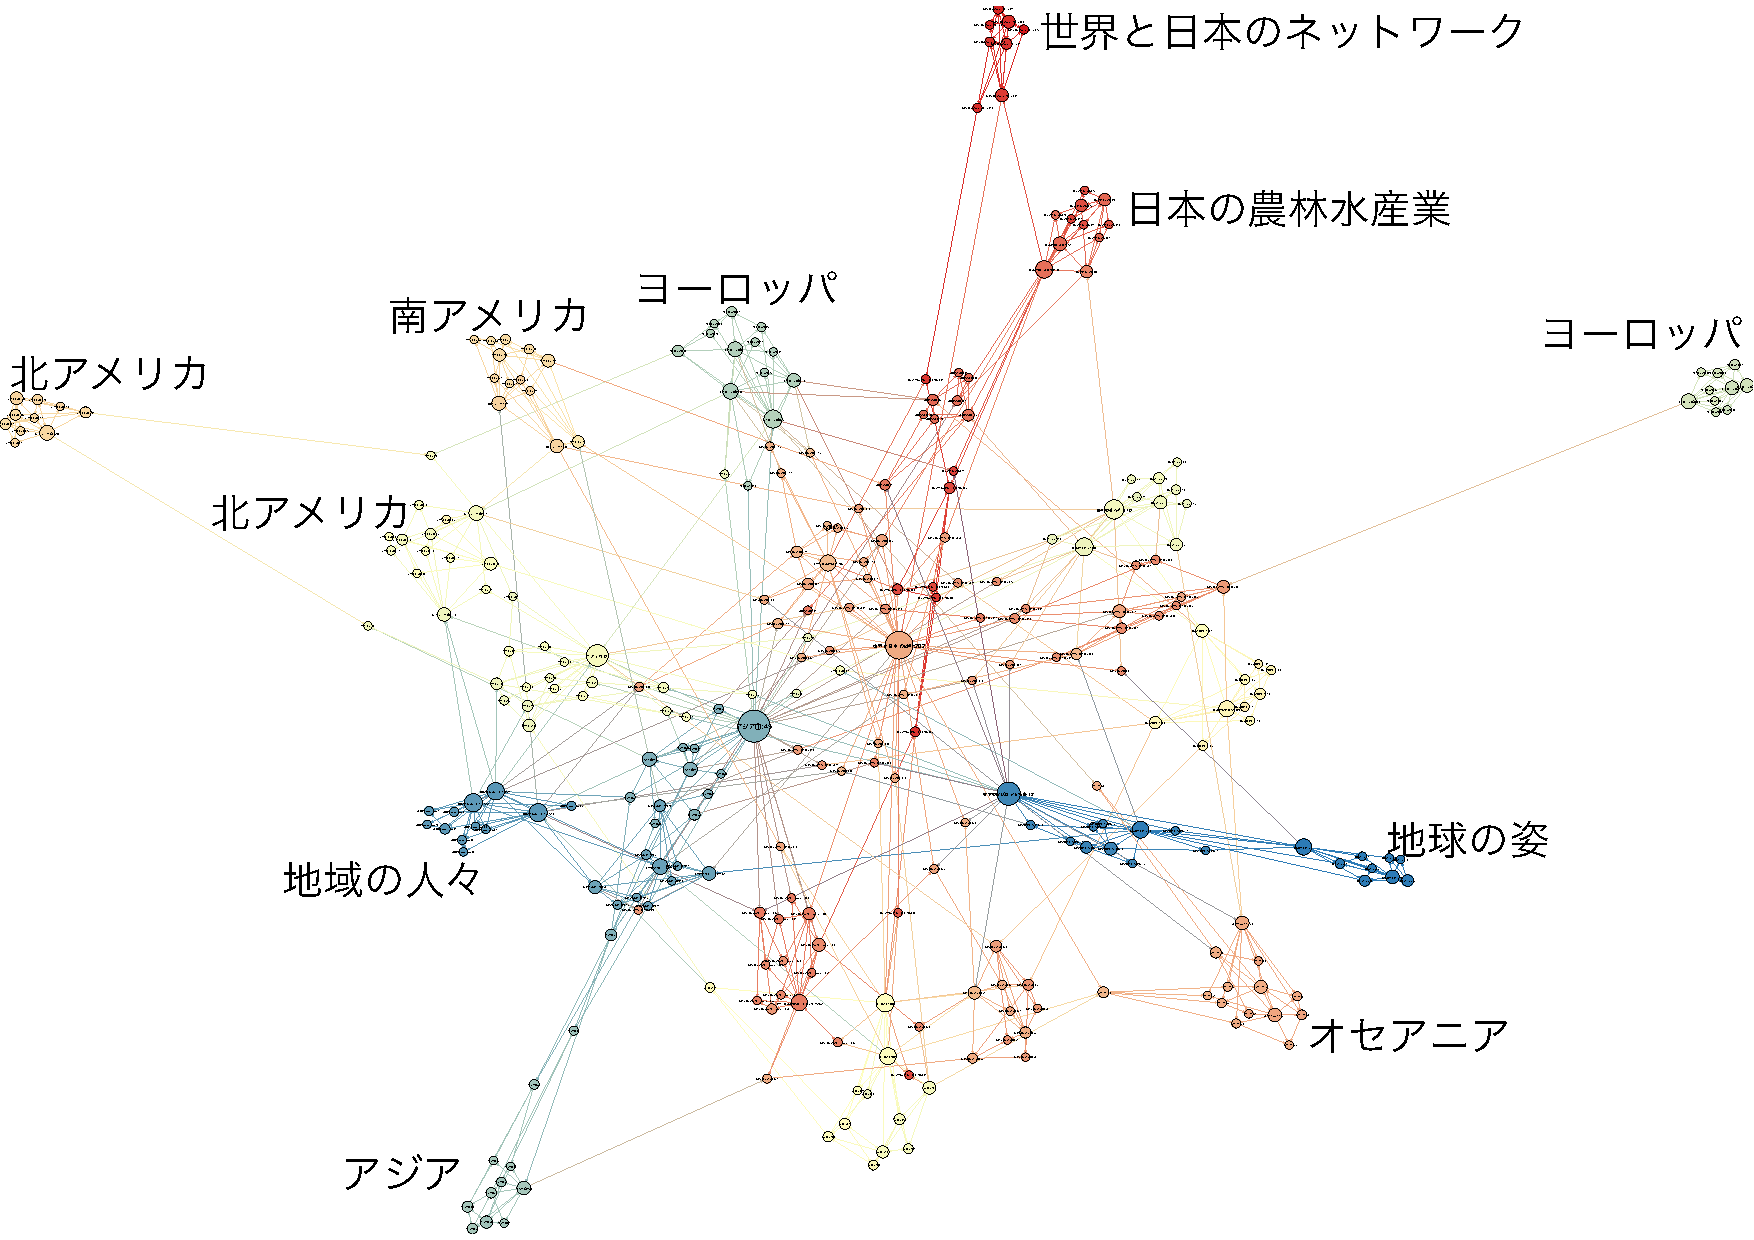
\includegraphics[width=330pt]{./img/c_geo_label2.pdf}
	\caption{中学地理の知識間関係ネットワーク}
	\label{fig:net_c_geo}
\end{center}
\end{figure}
中学地理のネットワークを図\ref{fig:net_c_geo}に示す.
多くのノードが内容ごとでクラスタを形成している.
特に,
ヨーロッパ,南アメリカ,アジア,オセアニア等,世界の各地域の内容はそれぞれでクラスタを形成している.
また,中央のオレンジから右上にかけて緩やかに結合しているノード群は日本あるいは日本と世界との関連についての内容となっている.





\subsubsection{中学歴史}
\begin{figure}[!htb]
\begin{center}
	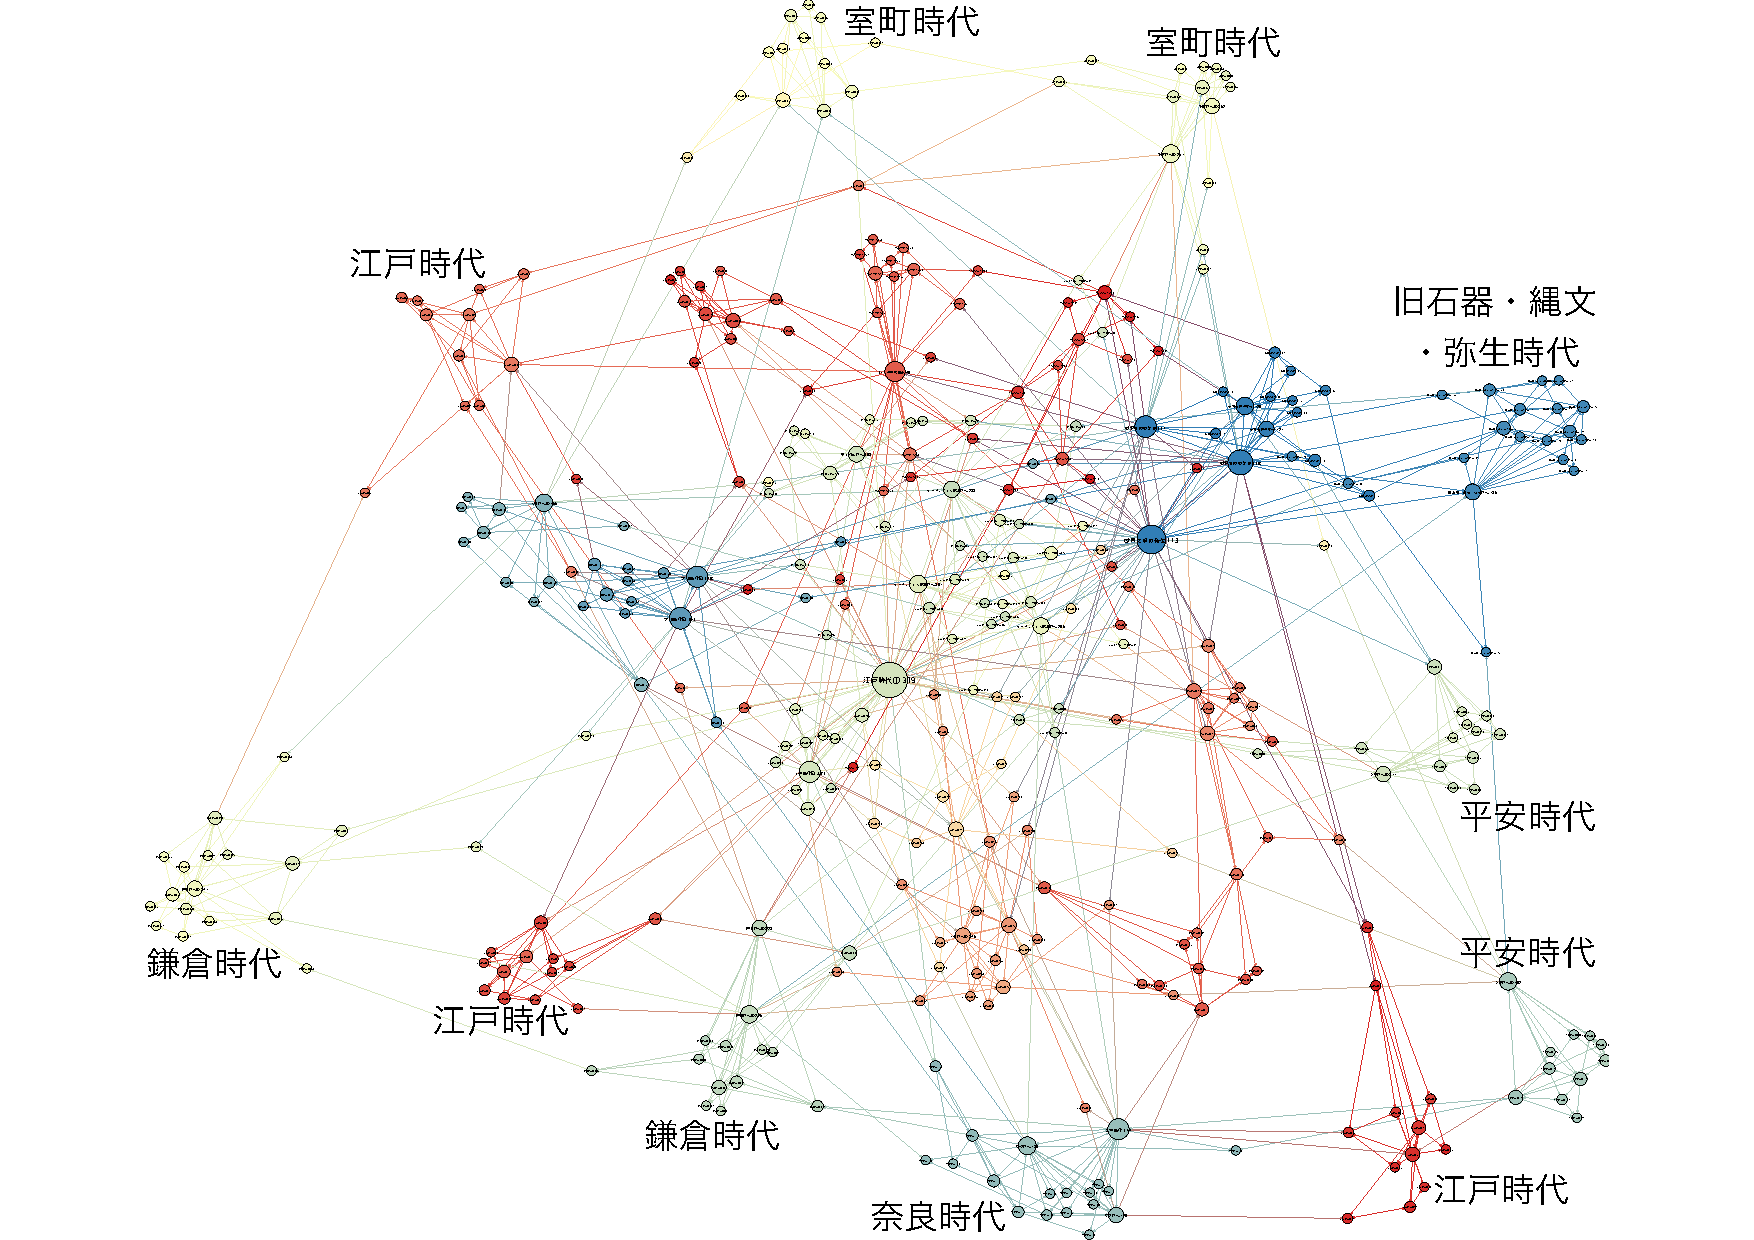
\includegraphics[width=330pt]{./img/c_his_label2.pdf}
	\caption{中学歴史の知識間関係ネットワーク}
	\label{fig:net_c_his}
\end{center}
\end{figure}
中学歴史のネットワークを図\ref{fig:net_c_his}に示す.
多くのノードが内容ごとでクラスタを形成している一方で,中央にノードが雑多な形で集まっている.
中央の雑多なノード群は主に安土桃山時代,江戸時代,ルネサンス時代,大航海時代,市民革命,産業革命等に関するものであるが,
日本の安土桃山時代(1573年から1603年),江戸時代(1603年から1867年)の年代と,
欧米諸国の
ルネサンス時代(14世紀から16世紀),大航海時代(15世紀から17世紀),市民革命(18世紀),産業革命(18世紀から19世紀)
の年代が概ね合致していることが興味深い.




次に,
手続き的的知識について知識間関係ネットワークを順に可視化していく.

\subsubsection{小学4年算数}
\begin{figure}[!htb]
\begin{center}
	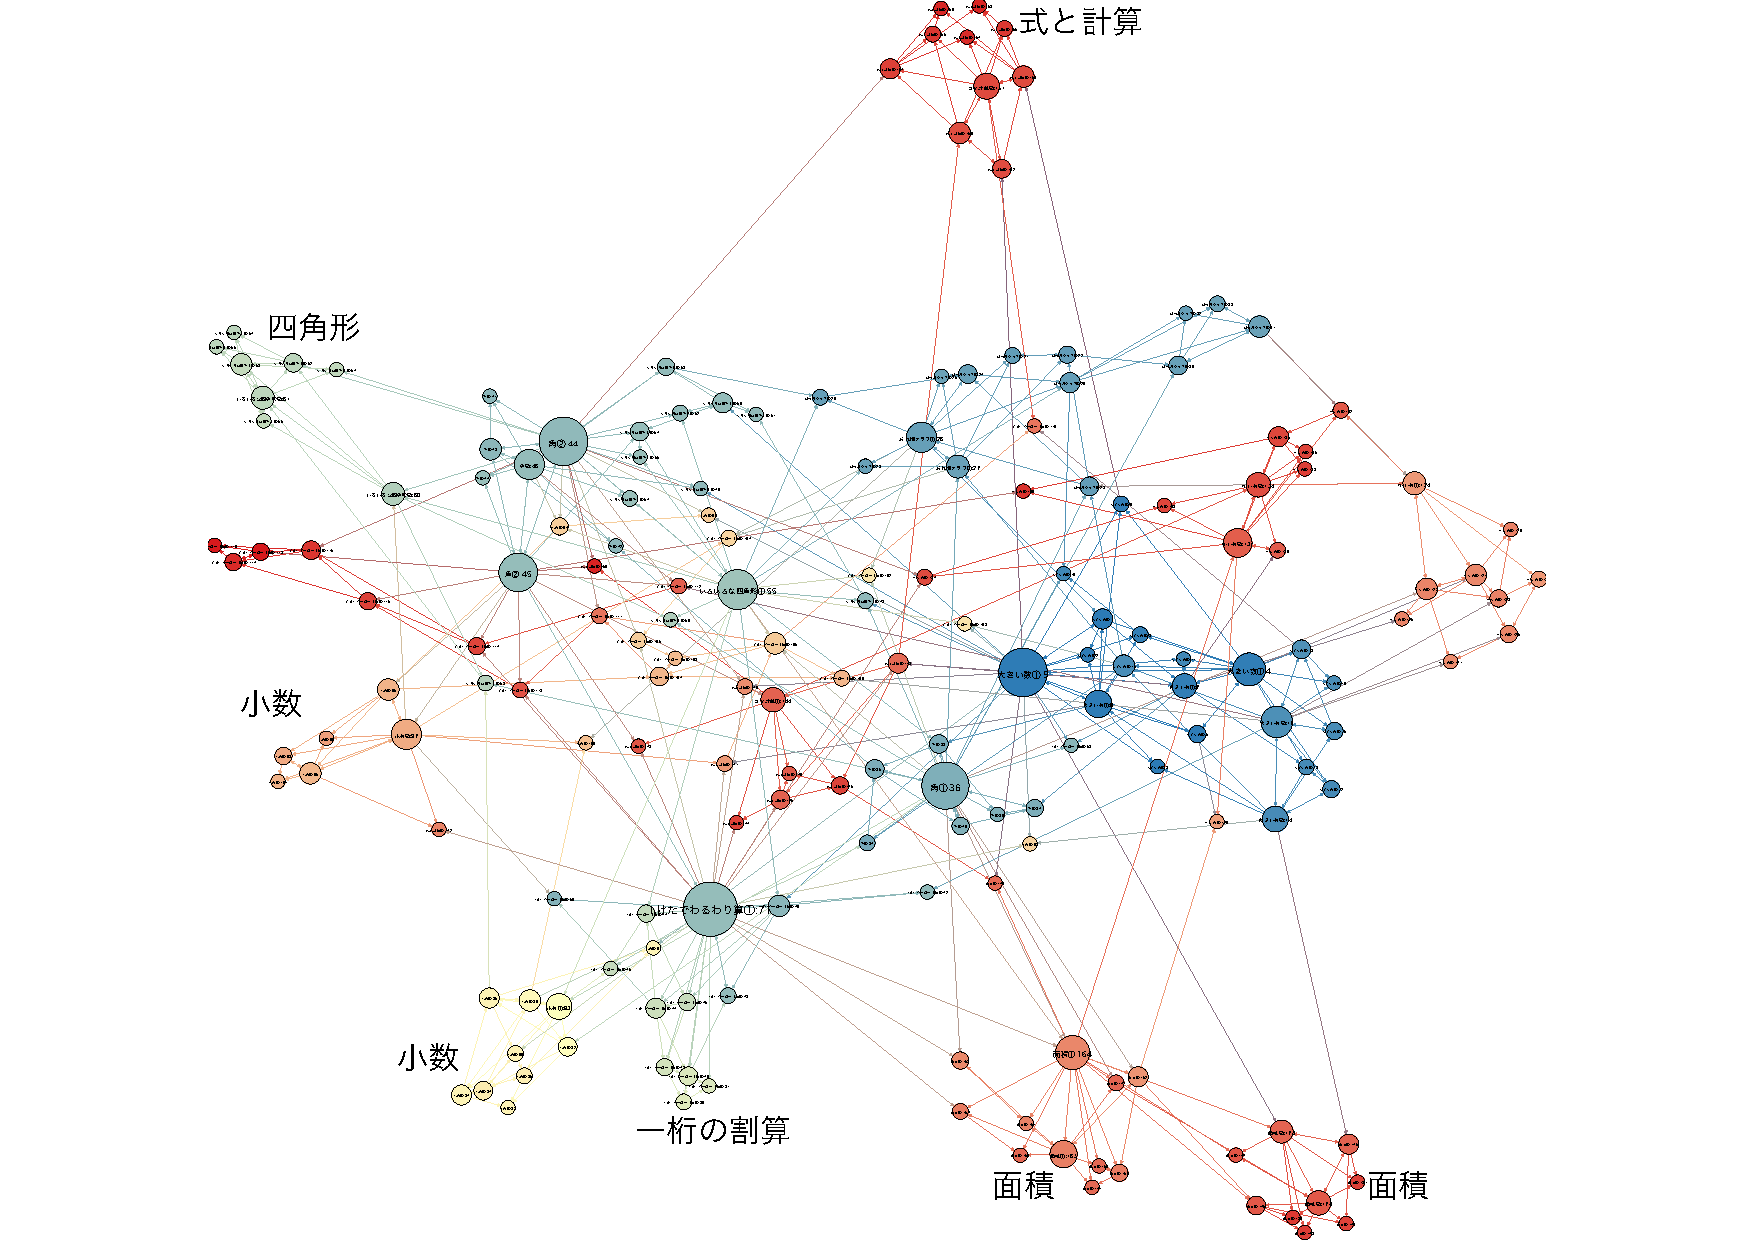
\includegraphics[width=330pt]{./img/s4_mat_label2.pdf}
	\caption{小学4年算数の知識間関係ネットワーク}
	\label{fig:net_s4mat}
\end{center}
\end{figure}
小学4年算数のネットワークを図\ref{fig:net_s4mat}に示す.
一部のノードがクラスタを形成している.
小学4年社会や小学5年社会のネットワークと比べると,クラスタの形成度合いは小さいように見られる.
特に,青色のノードが中央に寄っていて,外側に出ているノードはオレンジや赤色のノードが多いことも1つの特徴であると考えられる.
このことは,着手される順序が遅い問題の方がネットワークの中心になく,つまり影響を与える問題が少ないことを示唆している.





\subsubsection{小学5年算数}
\begin{figure}[!htb]
\begin{center}
	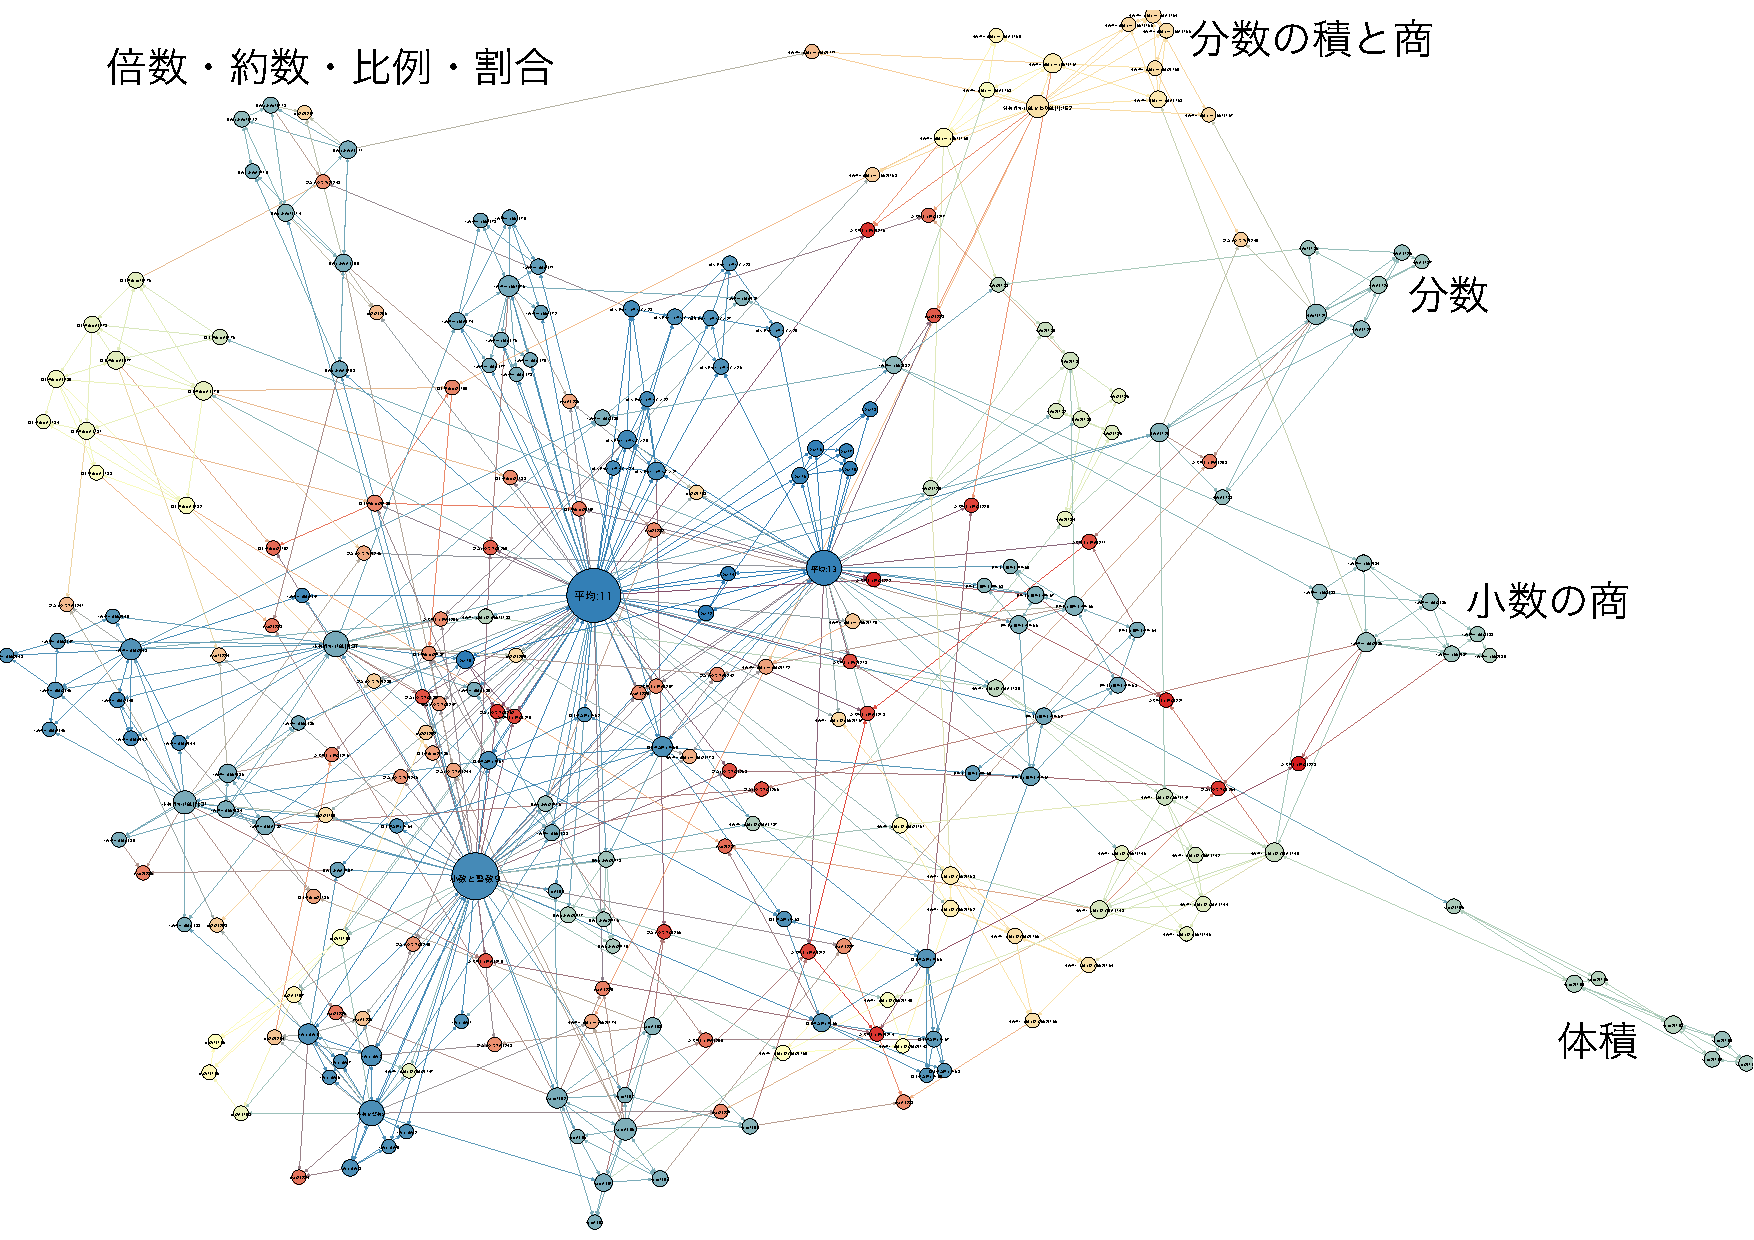
\includegraphics[width=330pt]{./img/s5_mat_label2.pdf}
	\caption{小学5年算数の知識間関係ネットワーク}
	\label{fig:net_s5mat}
\end{center}
\end{figure}
小学5年算数のネットワークを図\ref{fig:net_s5mat}に示す.
全体としてノードは複雑に結合しており,モジュール性は低そうである.
また,ごく一部のノードが他のノードと比べて大きく,つまり,出力次数が大きい.
このことは,これらの大きいノードによって表現される知識は多くの知識の獲得に影響を与えていることを示唆している.
特に,大きいノードは平均や小数,整数に関する問題で,かつ,着手順序が早いものであることも大きな特徴である.
クラスタという観点では,小さなクラスタを形成しているノード群は小数や分数,あるいは体積に関するノードであることが特徴的である.



\subsubsection{小学6年算数}
\begin{figure}[!htb]
\begin{center}
	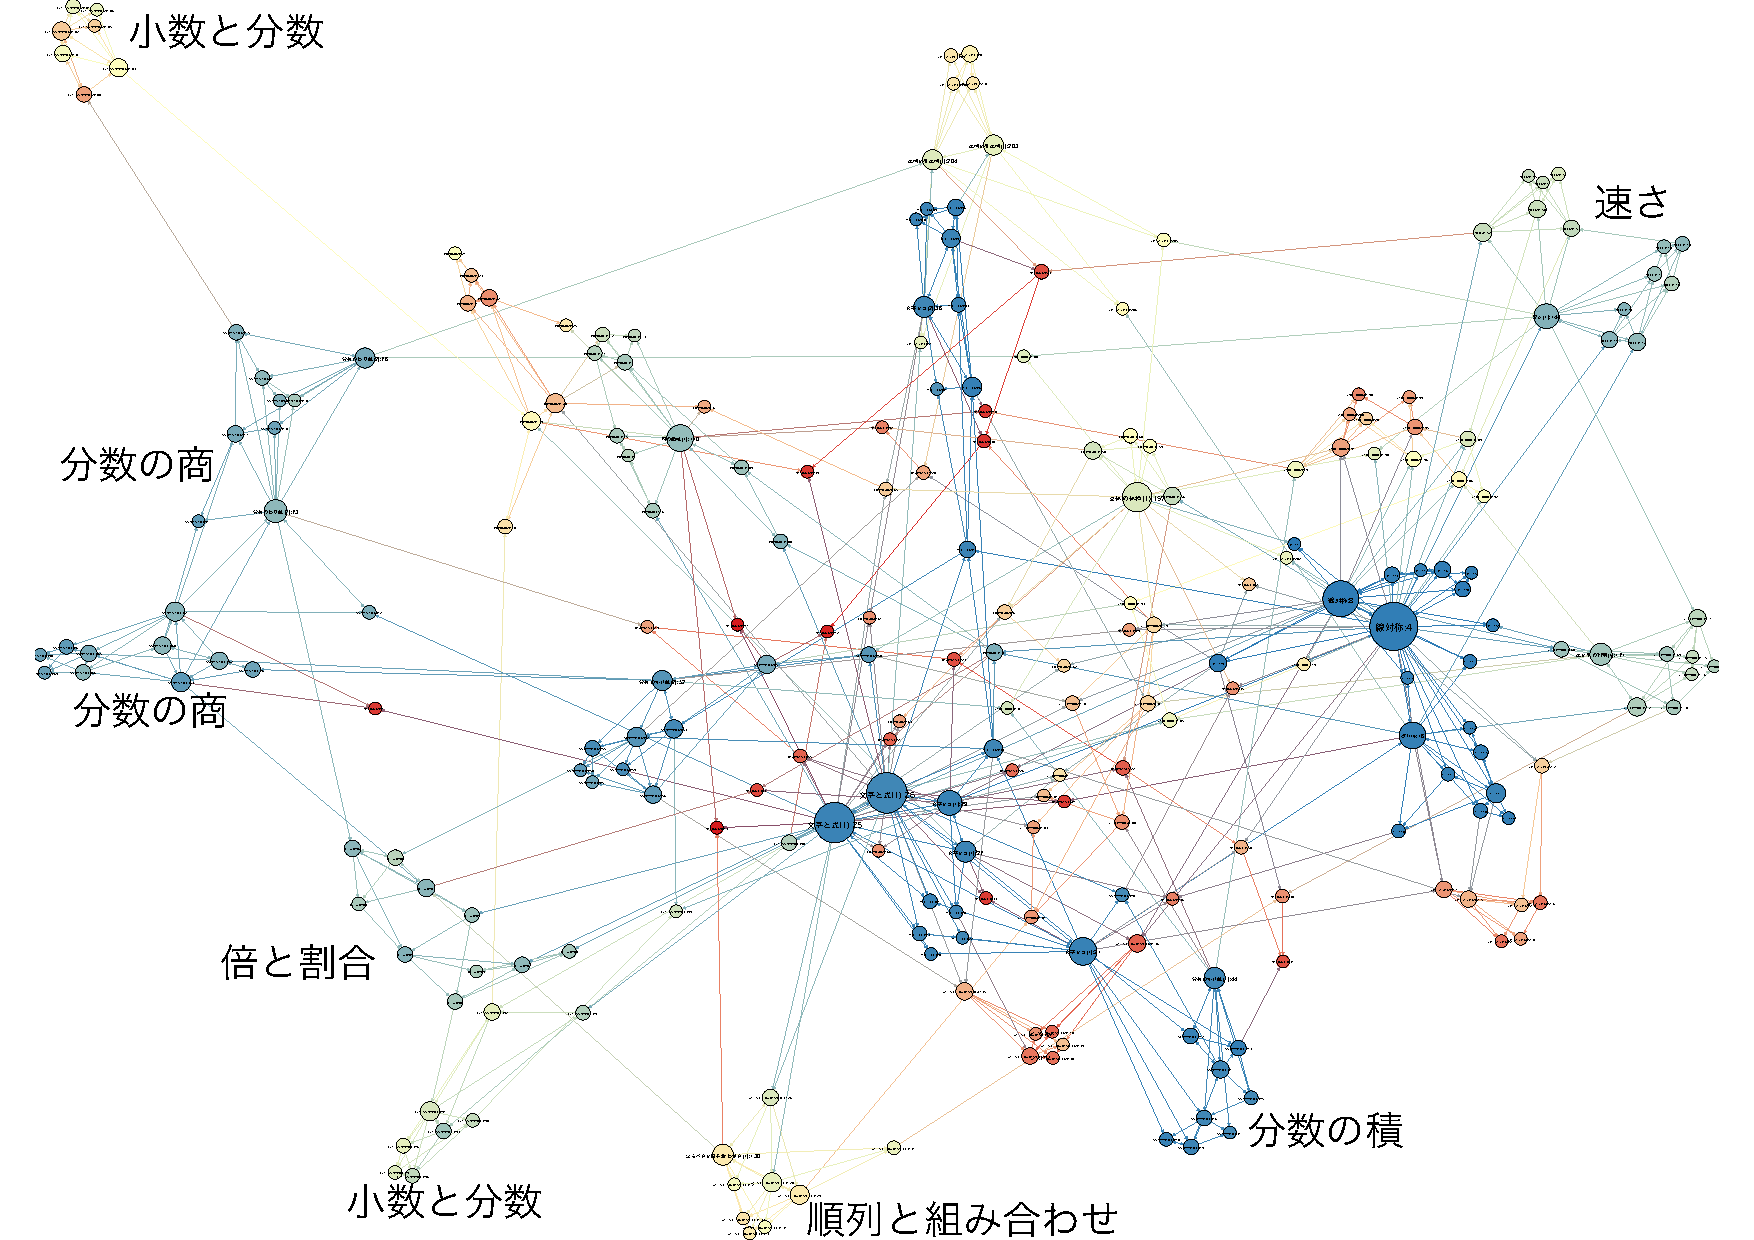
\includegraphics[width=330pt]{./img/s6_mat_label2.pdf}
	\caption{小学6年算数の知識間関係ネットワーク}
	\label{fig:net_s6mat}
\end{center}
\end{figure}
小学6年算数のネットワークを図\ref{fig:net_s6mat}に示す.
全体としてノードは複雑に結合しているが,一方で一部は小さなクラスタを形成している.
特にクラスタを形成するノード群の内容は
左のクラスタのノード群が小数や分数,それらの積や商の活用が求められる内容で,
下のクラスタのノード群が順列と組み合わせに関する内容で,
右上のクラスタのノード群が速さに関する内容となっている.
また,中央のごく一部ノードが青色で他のノードと比べて大きいことも大きな特徴である.
このことは,最初に獲得した知識が他の多くの知識の獲得に影響をもつことを示唆している.




\subsubsection{中学1年数学}
\begin{figure}[!htb]
\begin{center}
	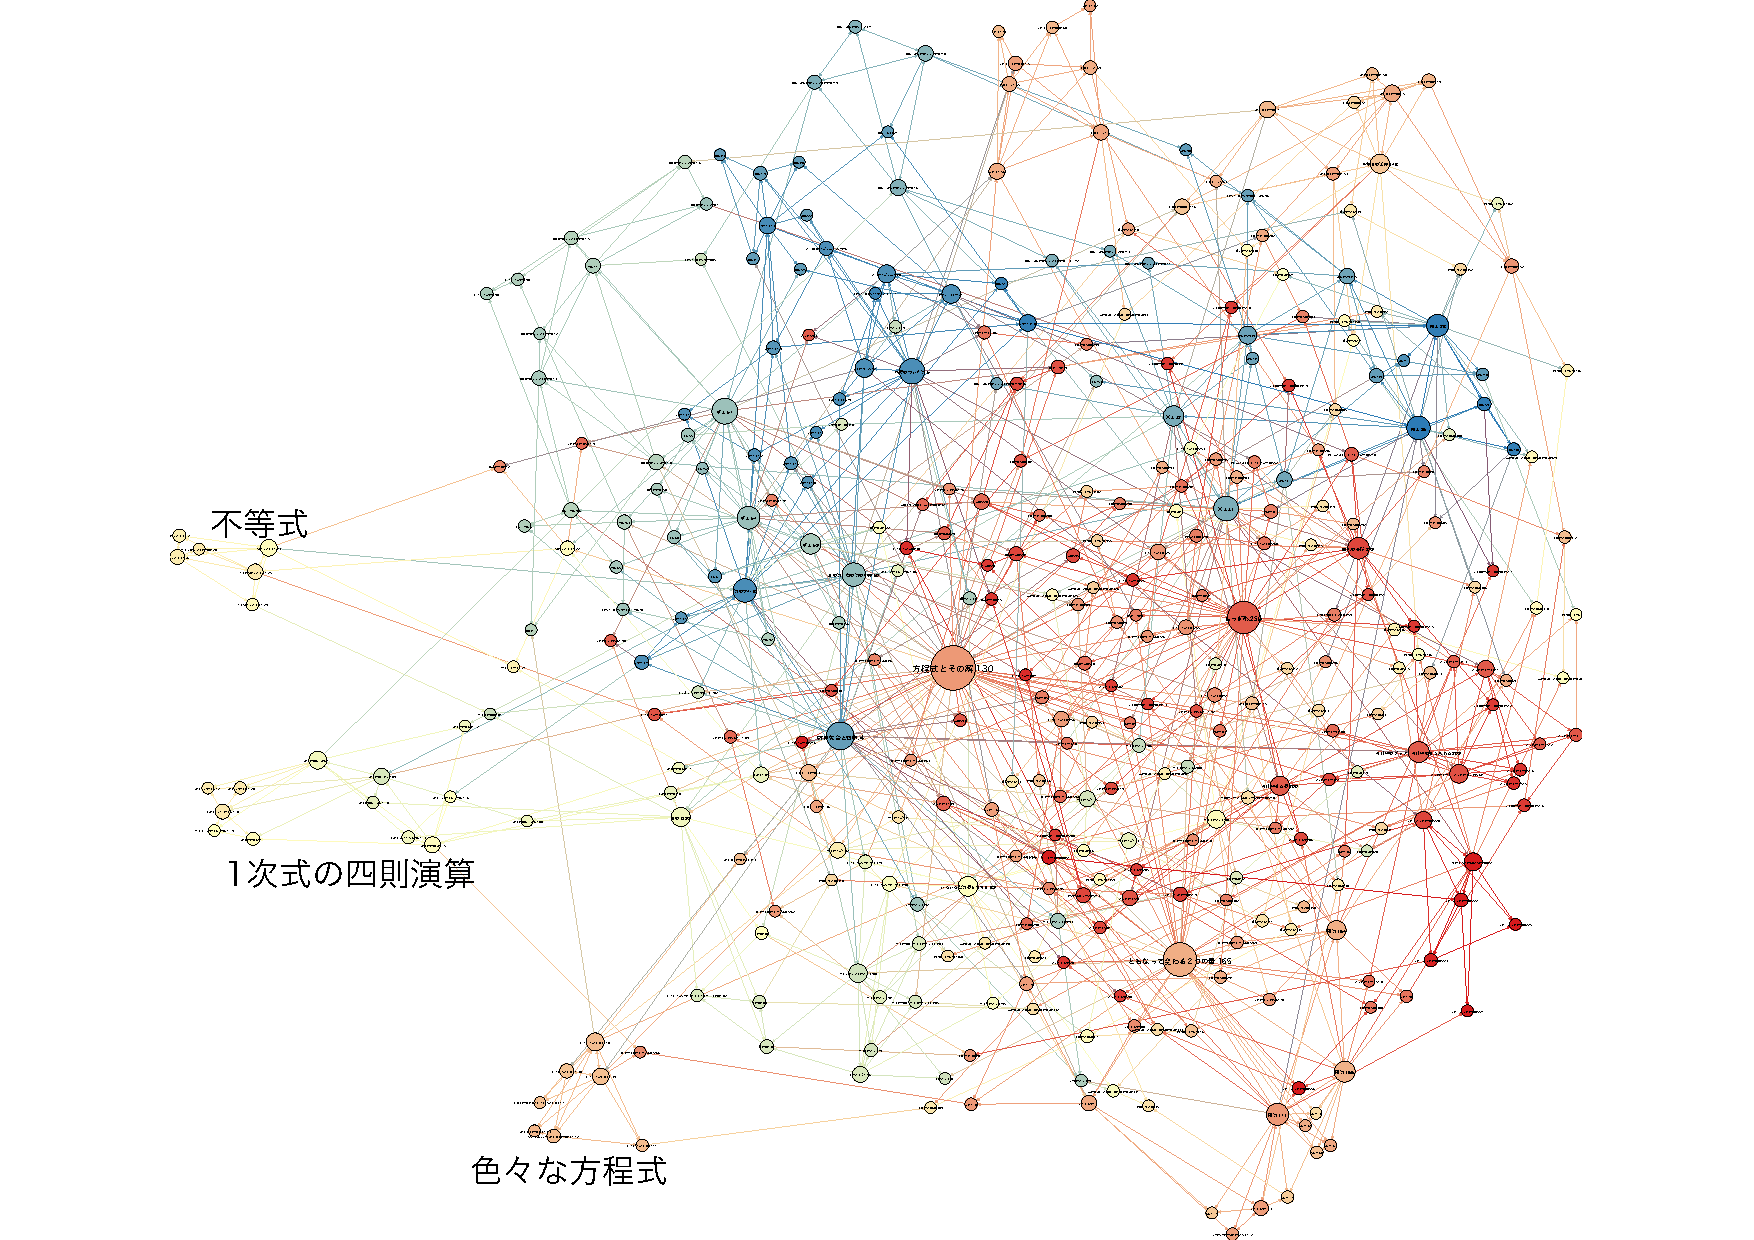
\includegraphics[width=330pt]{./img/c1_mat_label2.pdf}
	\caption{中学1年数学の知識間関係ネットワーク}
	\label{fig:net_c1mat}
\end{center}
\end{figure}
中学1年数学のネットワークを図\ref{fig:net_c1mat}に示す.
全体としてノードは複雑に結合しており,小さなクラスタはほとんど存在しない.
特筆すべき点は中央オレンジ色の「方程式とその解」の内容を扱うノードが非常に大きく,出力次数が大きいことである.
このことは,方程式とその解に関する知識が中学1年数学の学習において非常に重要な位置付けにあることを示唆している.
小さなクラスタを形成しているノード群は
不等式,1次式の四則演算,色々な方程式に関する内容を扱うものであった.





\subsubsection{中学2年数学}
\begin{figure}[!htb]
\begin{center}
	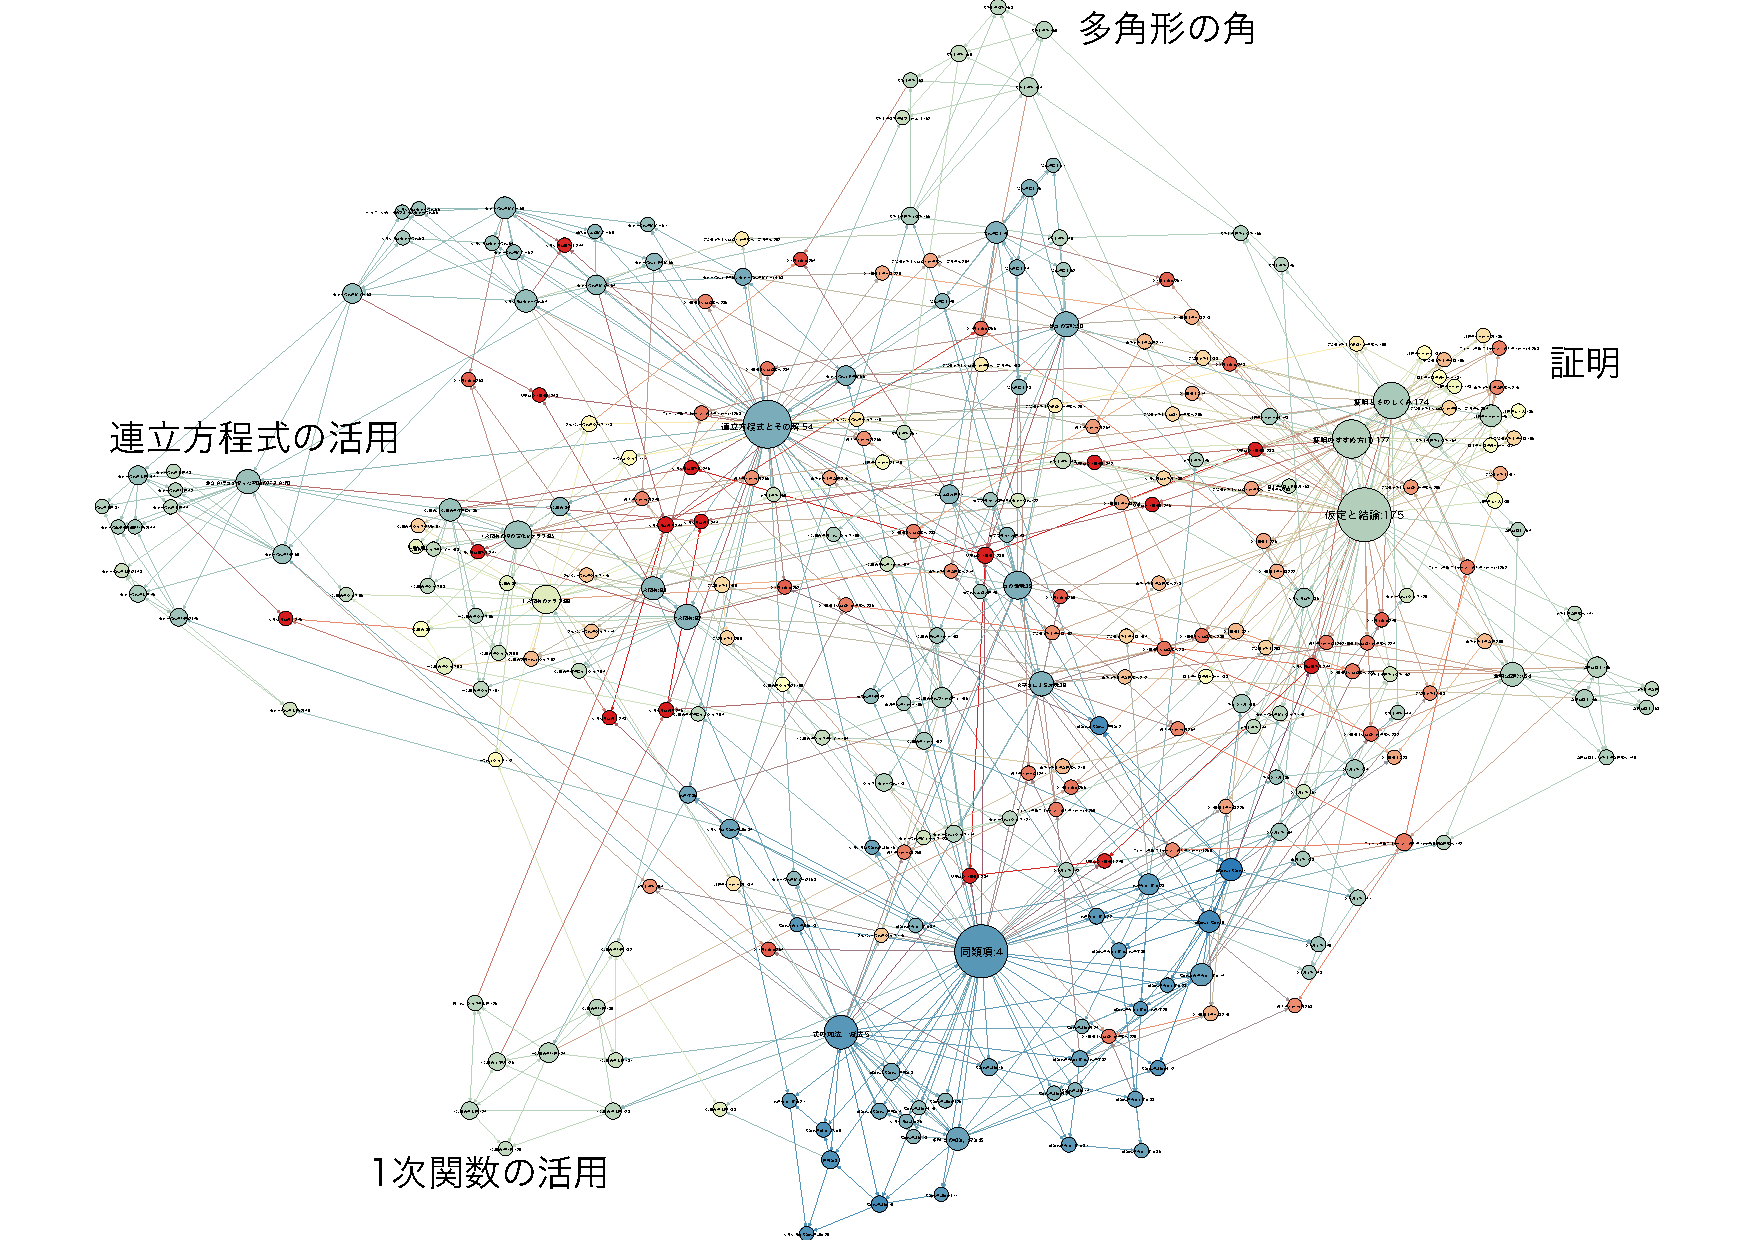
\includegraphics[width=330pt]{./img/c2_mat_label2.pdf}
	\caption{中学2年数学の知識間関係ネットワーク}
	\label{fig:net_c2mat}
\end{center}
\end{figure}
中学2年数学のネットワークを図\ref{fig:net_c2mat}に示す.
全体としてノードは密に結合しているものの,一部で緩やかにクラスタを形成している.
連立方程式の活用や1次関数の活用がクラスタとなっている.活用に関する知識は,ある種の特殊な事例を扱うためほかへの適用可能性が低く,結果としてモジュール性が高い可能性がある.
また,右上の大きなノードが仮定や結論,証明に関する内容を扱うものであり,またその近傍にあるノード群が三角形の合同証明,2線の並行証明等,証明の活用事例に関する内容を扱うものであることも興味深い.
証明という一般的な手続き的知識が合同や並行への理解に大きな影響を与えることを示唆している.





\subsubsection{中学3年数学}
\begin{figure}[!htb]
\begin{center}
	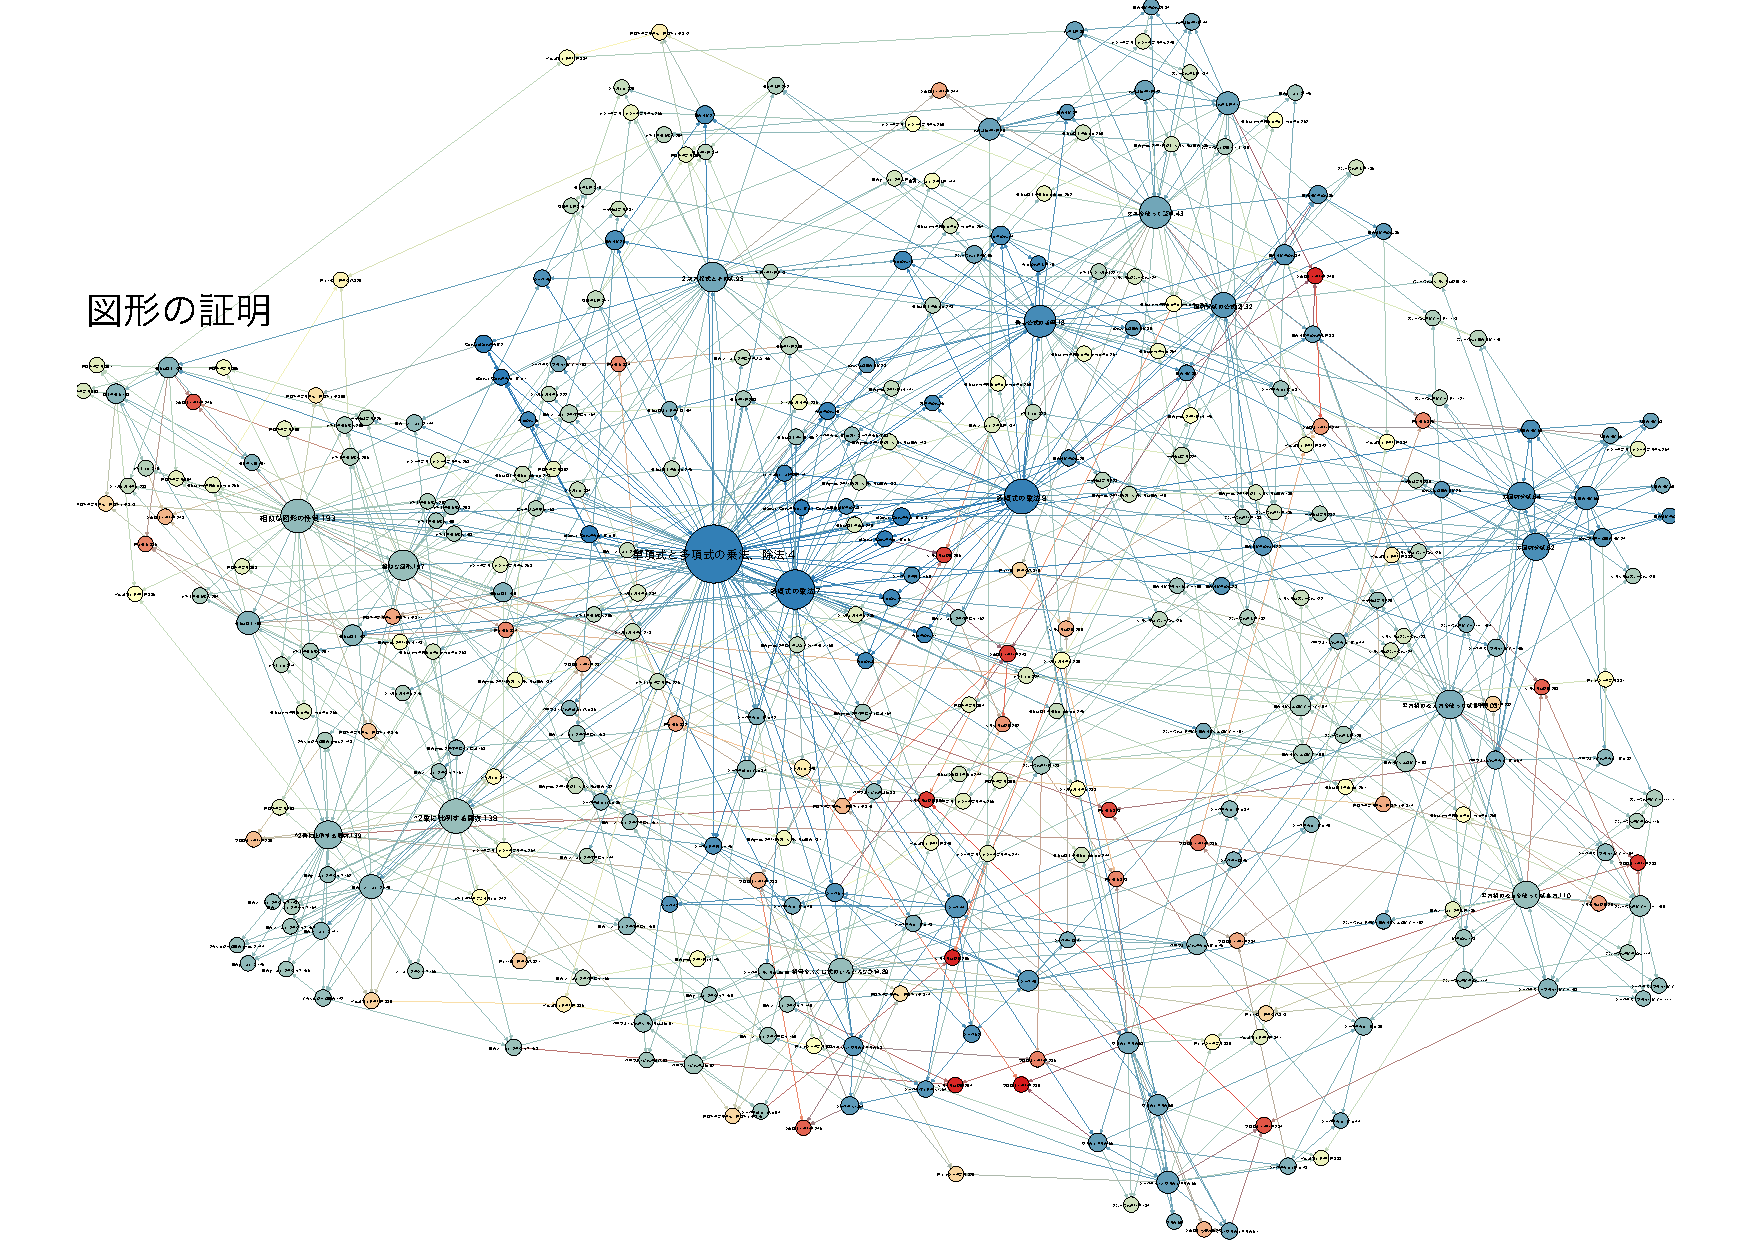
\includegraphics[width=330pt]{./img/c3_mat_label2.pdf}
	\caption{中学3年数学の知識間関係ネットワーク}
	\label{fig:net_c3mat}
\end{center}
\end{figure}
中学3年数学のネットワークを図\ref{fig:net_c2mat}に示す.
全体としてノードは複雑に結合しており,一部が密になっているというようなクラスタはほとんど存在しない.
中央の青色のノードが非常に大きく,出力次数が大きい.
このノードは単項式と多項式の乗法除法に関する内容を扱うものであり,
したがって,中学3年数学において単項式と多項式に乗法除法に関する知識は非常に重要な位置付けにあることを示唆している.



以上,個々の知識間関係ネットワークを可視化した.
全体として,ノードは内容の関連度が大きいノードと結合しており,
これらのネットワークは,
確かに,
知識獲得における知識構造を表現しているものと考えられる.


\subsection{ネットワーク構造の分析}

\begin{table}[!htb]
\caption{各ネットワークにおける構造指標}
\label{tab:result2}
\begin{center}
\centerline{
{
\begin{tabular}{ccc|cc|cc|cc}\hline\hline
\multicolumn{3}{c|}{ネットワーク}	&	\multicolumn{2}{c|}{モジュラリティ}	& \multicolumn{2}{c|}{フロー階層}	&\multicolumn{2}{c}{GRC}		\\
	分類	& 科目			&				学年			&		値		&	平均			&	値		&	平均	&	値	&	平均	\\\hline
\multirow{5}{*}{\shortstack{宣言的知識\\の知識間関係\\ネットワーク}}&	\multirow{3}{*}{地理・社会}		&		小学4年			&	0.698	&	\multirow{5}{*}{0.759}&	0.579		&	\multirow{5}{*}{0.627}	&	0.787		& \multirow{5}{*}{0.690}\\
		&				&	小学5年						&	0.801	&	&	0.541	&	&	0.679		&			\\
		&				&				中学			&	0.759	&	&	0.633	&	&	0.603		&			\\\cdashline{2-3}
		&\multirow{2}{*}{歴史・社会}	&	小学6年		&	0.808	&	&	0.607	&	&	0.613		&			\\
		&				&				中学			&	0.728	&	&	0.774	&	&	0.768		&			\\\hdashline
%
\multirow{6}{*}{\shortstack{手続き的知識\\の知識間関係\\ネットワーク}}&		\multirow{6}{*}{算数・数学}&	小学4年			&	0.660	&	\multirow{6}{*}{0.602}	&	0.590	&	\multirow{6}{*}{0.756}	&	0.683	&	\multirow{6}{*}{0.816} \\
		&				&				小学5年			&	0.602	&	&	0.757	&	&	0.901	&			\\
		&				&				小学6年			&	0.688	&	&	0.705	&	&	0.875	&			\\
		&				&				中学1年			&	0.566	&	&	0.805	&	&	0.803	&			\\
		&				&				中学2年			&	0.559	&	&	0.830	&	&	0.818	&			\\
		&				&				中学3年			&	0.538	&	&	0.847	&	&	0.861	&			\\
%
\hline\hline
\end{tabular}
}
}
\end{center}
\end{table}

%0.602	&	0.757	&	0.901	&	&	&
%0.688	&	0.705	&	0.875	&	&	&
%0.566	&	0.805	&	0.803	&	&	&
%0.559	&	0.830	&	0.818	&	&	&
%0.538	&	0.847	&	0.861	&	&	&
宣言的知識の知識構造を表現する5つのネットワークと
手続き的知識の知識構造を表現する6つのネットワーク
のモジュラリティとフロー階層,GRCを算出し,
知識獲得における知識構造について,
宣言的知識のモジュール性が手続き的知識のモジュール性より統計的に有意に高く,
逆に,
手続き的知識の階層性が宣言的知識の階層性より統計的に有意に高いことを示す.





表\ref{tab:result2}に各ネットワークにおける各構造指標を整理した.
まず,モジュラリティについて,
いずれの宣言的知識の知識間関係ネットワークのモジュラリティも
いずれの手続き的知識の知識間関係ネットワークのモジュラリティよりも高かった.
また,特に,手続き的知識の知識間関係ネットワークにおいては,学年が高いほど,モジュラリティが低い傾向にあり,つまり,難易度が高いほど知識のモジュール性が低い傾向にあることを示唆している.
逆説的に,難易度がより高い問題とは扱われる知識のモジュール性がより低いということを示唆しているとも考えられる.
 

次に,フロー階層について,
手続き的知識の知識間関係ネットワークのフロー階層の平均は
宣言的知識の知識間関係ネットワークのフロー階層の平均と比べ,
高かった.
このことは,手続き的知識の知識構造の方が宣言的知識の知識構造よりも循環構造が少ないことを示唆している.
また,
手続き的知識と
宣言的知識に限らず,
フロー階層は学年が高いほど高い傾向にあり,
このことは,知識はその獲得の難易度が高いほど循環構造が少ない傾向にあるか,あるいは,
知識獲得の順序性が強い傾向にあることを示唆している.

最後に,GRCについて,
手続き的知識の知識間関係ネットワークのGRCの平均は
宣言的知識の知識間関係ネットワークのGRCの平均と比べ,
高かった.
これはフロー階層と同様である.
一方で,GRCにおいてはフロー階層で見られた学年の傾向は現れていないようである.

また,3つの指標において,
小学4年算数の知識間関係ネットワークの構造は他の学年の算数や数学の知識間関係ネットワークの構造とは大きく異なる.
具体的には,
小学4年算数の知識間関係ネットワークのモジュラリティは高く,フロー階層とGRCは低かった.

さらに,
宣言的知識の知識間関係ネットワークと手続き的知識の知識間関係ネットワークにおける
モジュラリティ,フロー階層,GRCそれぞれについて,
t検定を実施し統計的に有意な差があるかを検証した.
モジュラリティにおけるp値は$0.00106$で,
フロー階層におけるp値は$0.0482$で,
GRCにおけるp値は$0.0470$
であった.
したがって,いずれの指標においても有意水準$0.05$で有意な差が認められた.
このことは
知識獲得における知識構造について,
宣言的知識のモジュール性が手続き的知識のモジュール性より統計的に有意に高く,
逆に,
手続き的知識の階層性が宣言的知識の階層性より統計的に有意に高いことを示している.



%0.00106480939912
%0.0481565072097
%0.0470423694215






\vvspace
以上,実験について述べた.
次章では,考察について述べる.



